\chapter{AHTR Optimization Preliminary Work}
\label{chap:realm-demo}
% Main Gist 
% - Demonstrate OpenMC problem with REALM. 
% Structure 
% - realm demonstration of OpenMC Coupling for a toy problem. 
In this chapter, I demonstrates using \gls{REALM} to apply genetic algorithms 
to maximize $k_{eff}$ in a single \gls{AHTR} fuel slab. 
Then, I will discuss the preliminary work completed for \gls{AHTR} multiphysics 
simulations.
The \texttt{dissertation-results} Github repository contains all the scripts, 
results, and plots shown in this chapter \cite{chee_dissertation-results_2021}.

\section{REALM Optimization: Straightened AHTR Fuel Slab}
\subsection{Problem Definition}
This demonstration explores how inhomogeneous fuel distributions impact $k_{eff}$ 
compared with homogenous fuel distributions customary in most reactor designs. 
The reactor core explored is a straightened slab from the \gls{FHR} benchmark's
\gls{AHTR} design.
Figure \ref{fig:straightened_slab} illustrates the straightened fuel slab. 
\begin{figure}[]
    \centering
    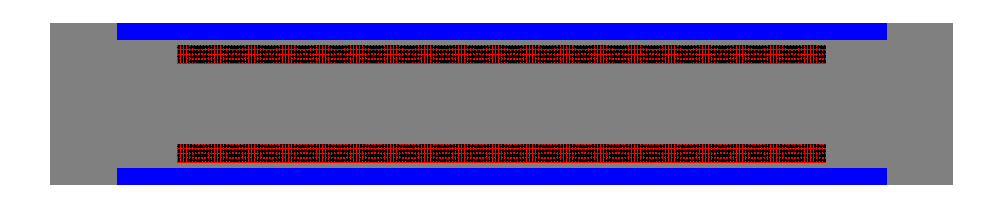
\includegraphics[width=\linewidth]{straightened_slab.png}
    \raggedright
    \resizebox{0.3\textwidth}{!}{
        \hspace{1cm}
        \fbox{\begin{tabular}{ll}
            \textcolor{fhrblue}{$\blacksquare$} & FLiBe \\
            \textcolor{fhrgrey}{$\blacksquare$} & Graphite (Fuel Plank)\\
            \textcolor{fhrred}{$\blacksquare$} & Graphite (Fuel Stripe) \\
            \textcolor{fhrblack}{$\blacksquare$} & TRISO particle 

            \end{tabular}}}
    \caption{Straightened \acrfull{AHTR} fuel slab.}
    \label{fig:straightened_slab}
\end{figure}
The slab has $27.1 \times 3.25 \times 1.85\ cm^3$ dimensions
with periodic boundary conditions in the x and y directions and reflective 
boundary conditions in the z-direction. 
The materials are the same as in the \gls{FHR} benchmark, except for 
the homogenization of each \gls{TRISO} particle's four outer layers: 
porous carbon buffer, inner pyrolytic carbon, silicon carbide layer, and the 
outer pyrolytic carbon. 
The \gls{TRISO} particles' dimensions remain the same.
Table \ref{tab:keff_triso} reports the $k_{eff}$ for this original straightened 
\gls{AHTR} configuration with and without the outer layer \gls{TRISO} 
homogenization.
\begin{table}[]
    \centering
    \onehalfspacing
    \caption{Straightened \acrfull{AHTR} fuel slab's $k_{eff}$ for case with 
    no \gls{TRISO} homogenization and case with homogenization of four outer 
    layers. Both simulations were run on one BlueWaters XE Node.}
	\label{tab:keff_triso}
    \footnotesize
    \begin{tabular}{llc}
    \hline 
    \textbf{TRISO Homogenization}& \textbf{$k_{eff}$} & \textbf{Simulation time [s]}  \\
    \hline 
    None & $1.38548 \pm 0.00124$ & 233\\ 
    4 outer layers & $1.38625 \pm 0.00109$ & 168\\ 
    \hline
    \end{tabular}
\end{table}
The \gls{TRISO} particle outer four layer homogenization resulted in a $30\%$ 
speed-up without compromising accuracy as both $k_{eff}$ values are within 
each other's uncertainty.

The \gls{REALM} optimization problem's objective is to maximize the slab's 
$k_{eff}$ by varying the \gls{TRISO} particle packing fraction across the slab
while keeping the total packing fraction constant at 0.0979. 
This total packing fraction is consistent with the original straightened slab with 
TRISO particles in fuel stripes (Figure \ref{fig:straightened_slab}). 
I divided the slab into ten slices along the x-axis between the \gls{FLiBe} and 
graphite buffers, resulting in ten $2.31 \times 2.55 \times 1.85\ cm^3$ slices. 
A sine distribution governs the \gls{TRISO} particle packing fraction's 
distribution across slices:
\begin{align}
    PF(x) &= \left(a\cdot sin(b\cdot x + c) + 2\right) \cdot NF\\
    \intertext{where}
    PF &= \mbox{packing fraction } [-] \nonumber \\ 
    a &= \mbox{amplitude, peak deviation of the function from zero } [-] \nonumber \\
    b &= \mbox{angular frequency, rate of change of the function argument } [\frac{radians}{cm}] \nonumber \\
    c &= \mbox{phase, the position in its cycle the oscillation is at t = 0 } [radians]\nonumber \\
    x &= \mbox{midpoint value for each slice } [cm]\nonumber \\
    NF &= \mbox{Normalization factor } [-]\nonumber
\end{align}
I collected and normalized the sine distribution's value at each of the ten 
x-slices' midpoints by the total packing fraction to ensure a consistent number 
of \gls{TRISO} particles in the slab.
For a packing fraction distribution of 
$PF(x) = \left(0.5\cdot sin(\frac{\pi}{3}\cdot x + \pi) + 2\right)  \cdot NF$, 
the packing fraction for the ten slices are 0.103, 0.120, 0.049, 0.138, 
0.076, 0.081, 0.136, 0.048, 0.125, and 0.098, respectively. 
Figure \ref{fig:triso_distribution} shows this sine distribution, highlights 
the packing fraction at the respective midpoints, and displays the slab's XY-view
with packing fraction varying based on this sine distribution. 
\begin{figure}[]
    \centering
    \makebox[\textwidth][c]{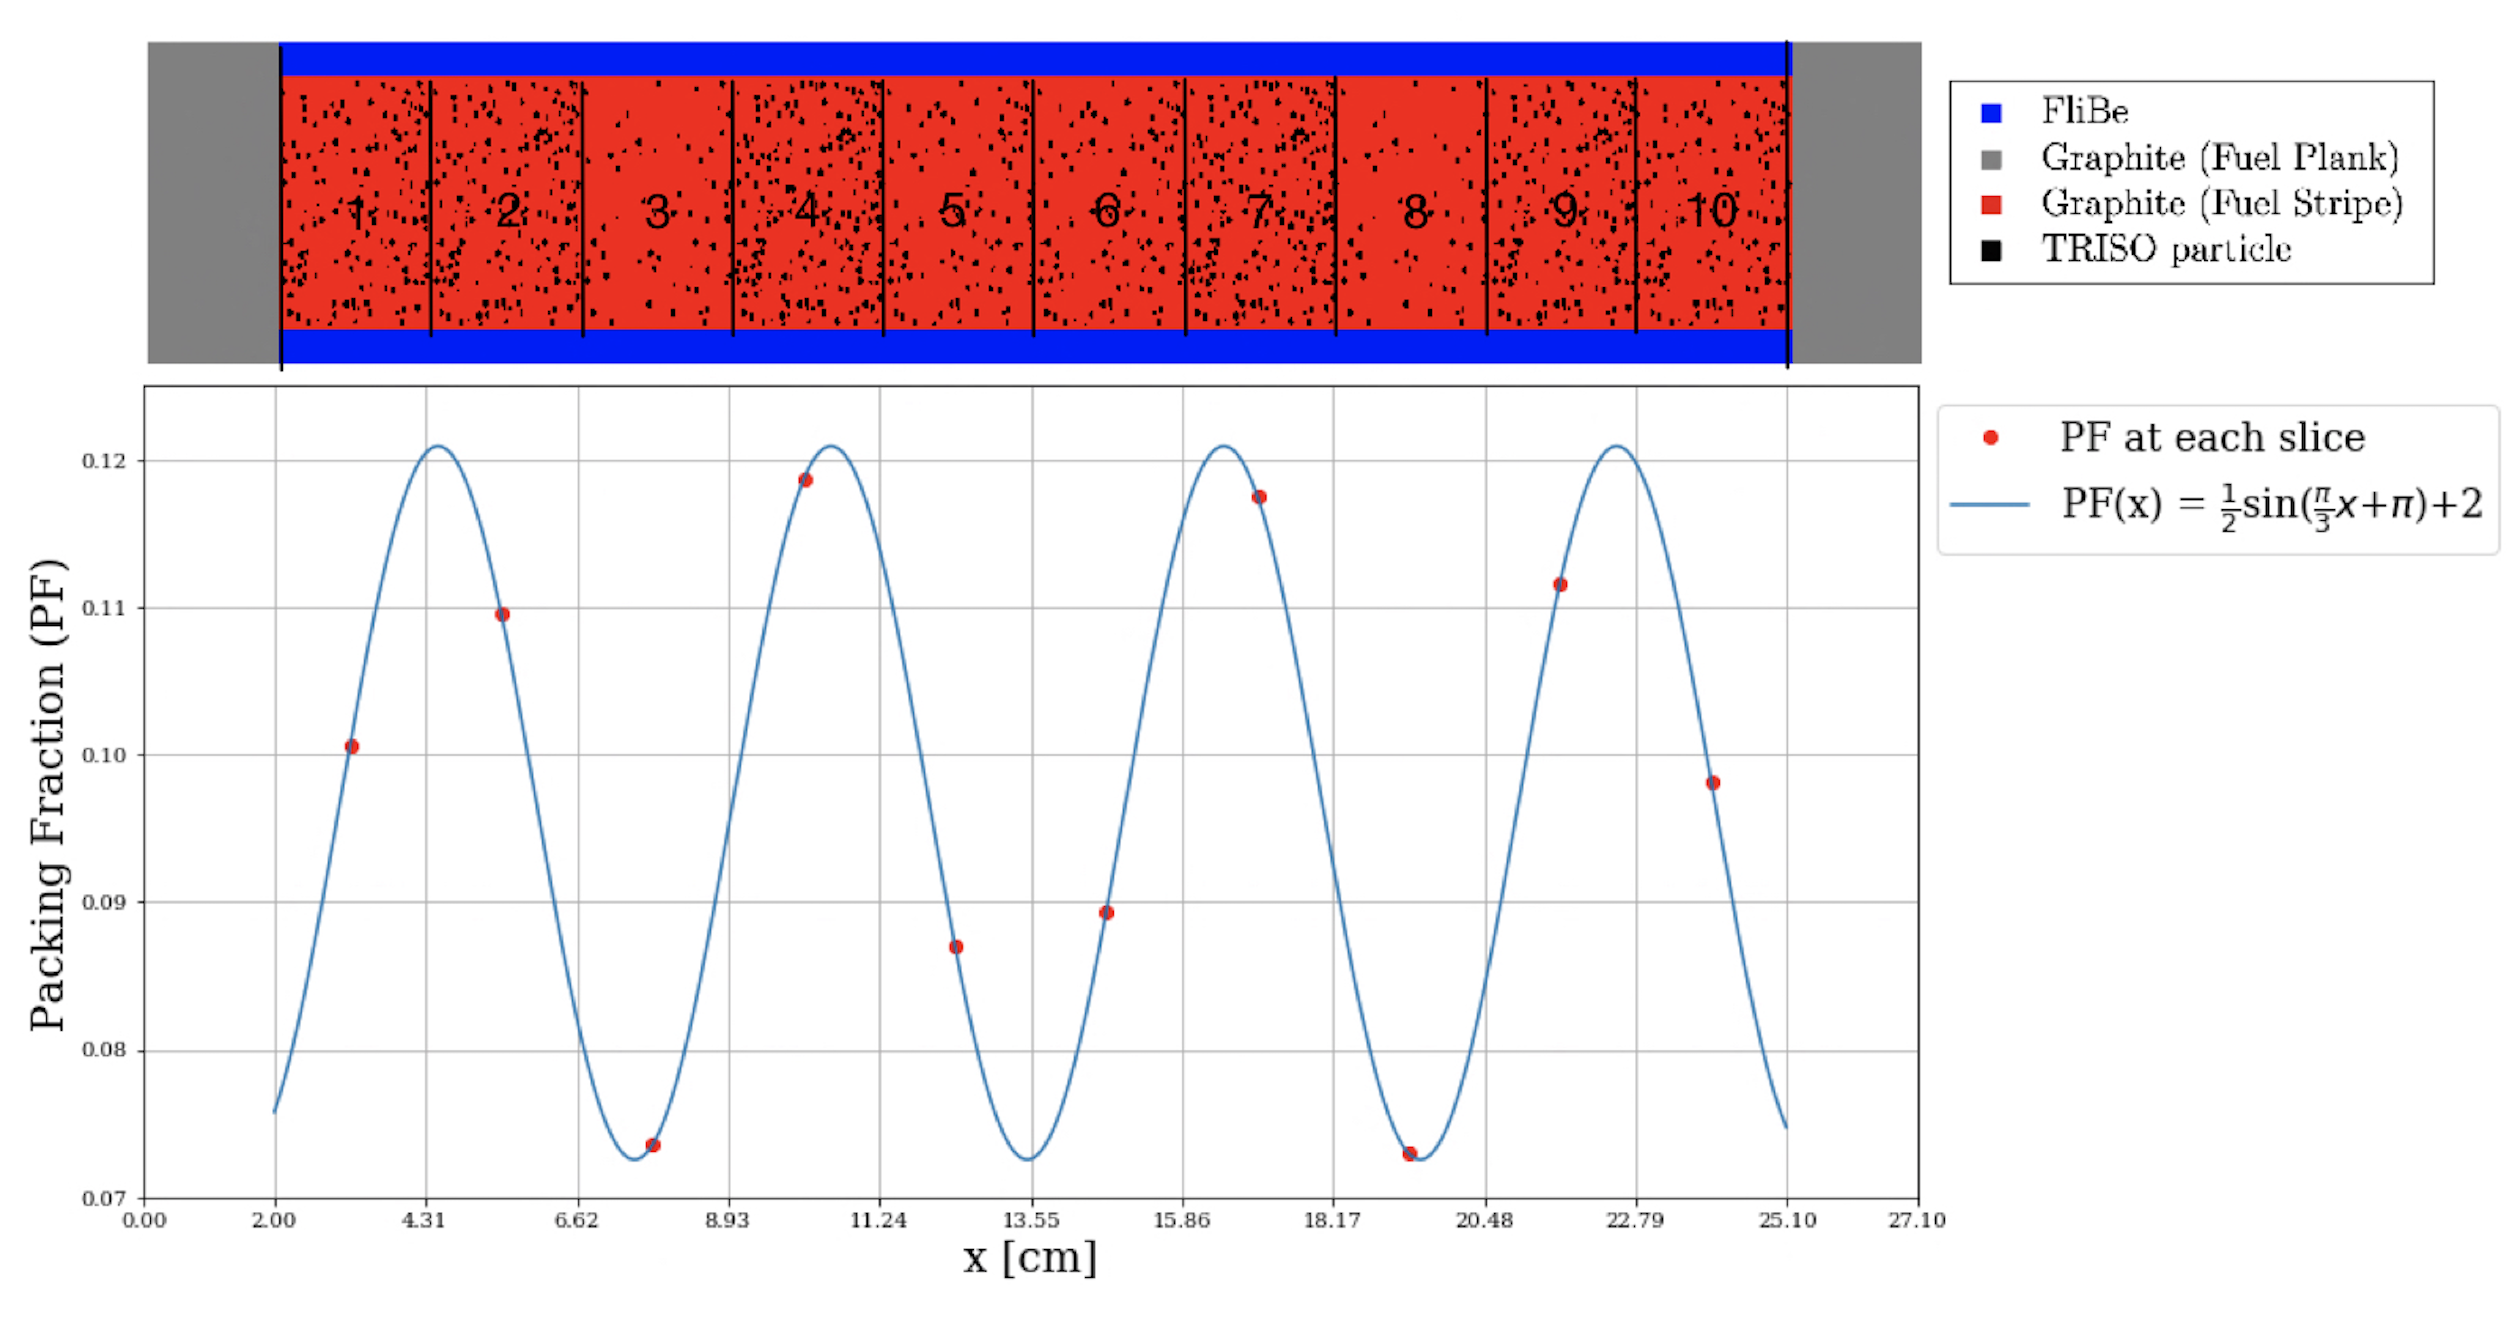
\includegraphics[width=1.1\linewidth]{triso_distribution_sine.png}} 
    \caption{Below: $PF(x) = (0.5\ sin(\frac{\pi}{3}x + \pi) + 2)  \times NF$ 
    sine distribution with red points indicating the packing fraction at each slice. 
    Above: Straightened \acrfull{AHTR} fuel slab with varying \gls{TRISO} particle 
    distribution across ten slices based on the sine distribution. }
    \label{fig:triso_distribution}
\end{figure}

In \gls{REALM}, a genetic algorithm varies the $a$, $b$, and $c$ variables to 
find a combination which produces a packing fraction distribution that maximizes 
the slab's $k_{eff}$. 
I defined the upper and lower bounds of $a$, $b$ and $c$ as: 
\begin{itemize}
    \item 0 $<$ $a$ $<$ 2 
    \item 0 $<$ $b$ $<$ $\frac{\pi}{2}$
    \item 0 $<$ $c$ $<$ $2\pi$
\end{itemize}
I selected $a$ variable's bounds to keep the sine distribution from falling 
below zero. 
The $b$ and $c$ variable bounds spread wide enough to allow the genetic 
algorithm to explore various sine distributions. 
The OpenMC evaluator calculates $k_{eff}$. 
OpenMC runs each simulation with 80 active cycles, 20 inactive cycles, and 
8000 particles to reach $\sim$130pcm uncertainty. 
Figure \ref{fig:realm-input-simple} shows the \gls{REALM} input file for this 
genetic algorithm optimization problem. 
\texttt{ahtr\_slab\_openmc.py} is the template OpenMC straightened \gls{AHTR} 
slab script that accepts $a$, $b$ and $c$ from \gls{REALM}, calculates packing 
fraction distribution, and assigns packing fraction values to each fuel slice. 
Subsequently, \gls{REALM} runs the templated OpenMC script to generate $k_{eff}$. 
\begin{figure}[]
    \begin{minted}[
        frame=lines,
        framesep=2mm,
        baselinestretch=1.2,
        fontsize=\footnotesize,
        linenos
        ]{json}
        {
            "control_variables": {
                "a": {"min": 0.0, "max": 2.0},
                "b": {"min": 0.0, "max": 1.57},
                "c": {"min": 0.0, "max": 6.28},
            },
            "evaluators": {
                "openmc": {
                    "input_script": "ahtr_slab_openmc.py",
                    "inputs": ["a", "b", "c"],
                    "outputs": ["keff"],
                    "keep_files": false,
                }
            },
            "constraints": {"keff": {"operator": [">="], "constrained_val": [1.0]}},
            "algorithm": {
                "objective": "max",
                "optimized_variable": "keff",
                "pop_size": 60,
                "generations": 10,
                "mutation_probability": 0.23,
                "mating_probability": 0.46,
                "selection_operator": {"operator": "selTournament", "k": 15, "tournsize": 5},
                "mutation_operator": {
                    "operator": "mutPolynomialBounded",
                    "eta": 0.23,
                    "indpb": 0.23,
                },
                "mating_operator": {"operator": "cxBlend", "alpha": 0.46},
            },
        }
        
    \end{minted}
    \caption{\acrfull{REALM} JSON input file to maximize $k_{eff}$ in the 
    straightened \acrfull{AHTR} fuel slab by varying packing fraction distribution 
    with control variables $a$, $b$, and $c$.}
    \label{fig:realm-input-simple}
\end{figure}

\subsection{Hyperparameter Search}
\label{sec:hyperparameter_search}
In \gls{REALM}'s input file, the user defines the genetic algorithm's 
hyperparameters. 
A good hyperparameter set guides the optimization process by 
balancing exploitation and exploration to find an optimal solution quickly 
and accurately. 
Finding a good set of hyperparameters requires a trial-and-error process. 

I performed the hyperparameter search with a coarse-to-fine random sampling scheme, 
whose advantages I previously discussed in Section \ref{sec:balance}.
The hyperparameters varied included population size, number of generations, 
mutation probability, mating probability, selection operator, selection operator's 
number of individuals, selection operator's tournament size, mutation operator, 
and mating operator.  
I started with 25 coarse experiments and fine-tuned the hyperparameters
with 15 more experiments. 
For each genetic algorithm experiment, I held the number of OpenMC evaluations 
constant at 600.
The number of evaluations correlated the population size and number of generations. 
I randomly sampled population size and used the following equation to calculate 
the number of generations: 
\begin{align}
    \mbox{no. of generations} &= \frac{\mbox{no. of evaluations}}{\mbox{population size} }
\end{align}
Table \ref{tab:hyperparameter_search} shows the lower and upper bounds used 
for each hyperparameter's random sampling. 
\begin{table}[]
    \centering
    \onehalfspacing
    \caption{Hyperparameter search is conducted in three phases: \textit{Coarse Search}, 
    \textit{Fine Search 1}, \textit{Fine Search 2}. Each hyperparameter's lower and
    upper bounds for each search phase are listed.}
	\label{tab:hyperparameter_search}
    \footnotesize
    \makebox[\textwidth][c]{\begin{tabular}{p{4cm}lp{3.4cm}p{3.4cm}p{3.4cm}}
    \hline 
    \textbf{Hyperparameter}& \textbf{Type} & \textbf{Coarse Search Bounds} & \textbf{Fine Search 1 Bounds} & \textbf{Fine Search 2 Bounds} \\
    \hline
    Experiments & - & 0 to 24 & 24 to 34 & 35 to 39 \\ 
    \hline
    Population size (pop) & Continuous & 10 $<$ x $<$ 100 & 20 $<$ x $<$ 60 & 60 \\ 
    Mutation probability & Continuous & 0.1 $<$ x $<$ 0.4 & 0.2 $<$ x $<$ 0.4& 0.2 $<$ x $<$ 0.3\\
    Mating probability & Continuous & 0.1 $<$ x $<$ 0.6 &  0.1 $<$ x $<$ 0.3 &  0.45 $<$ x $<$ 0.6\\
    Selection operator & Discrete & \texttt{SelTournament}, \texttt{SelBest}, \texttt{SelNSGA2} & \texttt{SelTournament}, \texttt{SelBest}, \texttt{SelNSGA2}& \texttt{SelTournament}\\
    Selection individuals & Continuous & $\frac{1}{3}pop$ $<$ x $<$ $\frac{2}{3}pop$ & $\frac{1}{3}pop$ $<$ x $<$ $\frac{2}{3}pop$ & 15\\
    Selection tournament size (only for SelTournament) & Continuous & 2 $<$ x $<$ 8 &2 $<$ x $<$ 8&5\\
    Mutation operator & Discrete & \texttt{mutPolynomialBounded} &\texttt{mutPolynomialBounded}&\texttt{mutPolynomialBounded}\\
    Mating operator & Discrete& \texttt{cxOnePoint}, \texttt{cxUniform}, \texttt{cxBlend} &\texttt{cxOnePoint}, \texttt{cxUniform}, \texttt{cxBlend}&\texttt{cxOnePoint}, \texttt{cxBlend}\\ 
    \hline
    \end{tabular}}
\end{table}

The initial 25 coarse experiments' sought to narrow down the hyperparameters 
to find a smaller set of optimal hyperparameter bounds that produce higher final 
generation $k_{eff}$ values.
Figure \ref{fig:hyperparameter_sens} shows the hyperparameters' plotted against 
each other with a third color dimension representing the $k_{eff ave}$ 
value in each experiment's final generation. 
Lighter scatter points indicate higher final population $k_{eff ave}$ values 
which suggests better hyperparameter sets. 
\begin{figure}[]
    \centering
    \makebox[\textwidth][c]{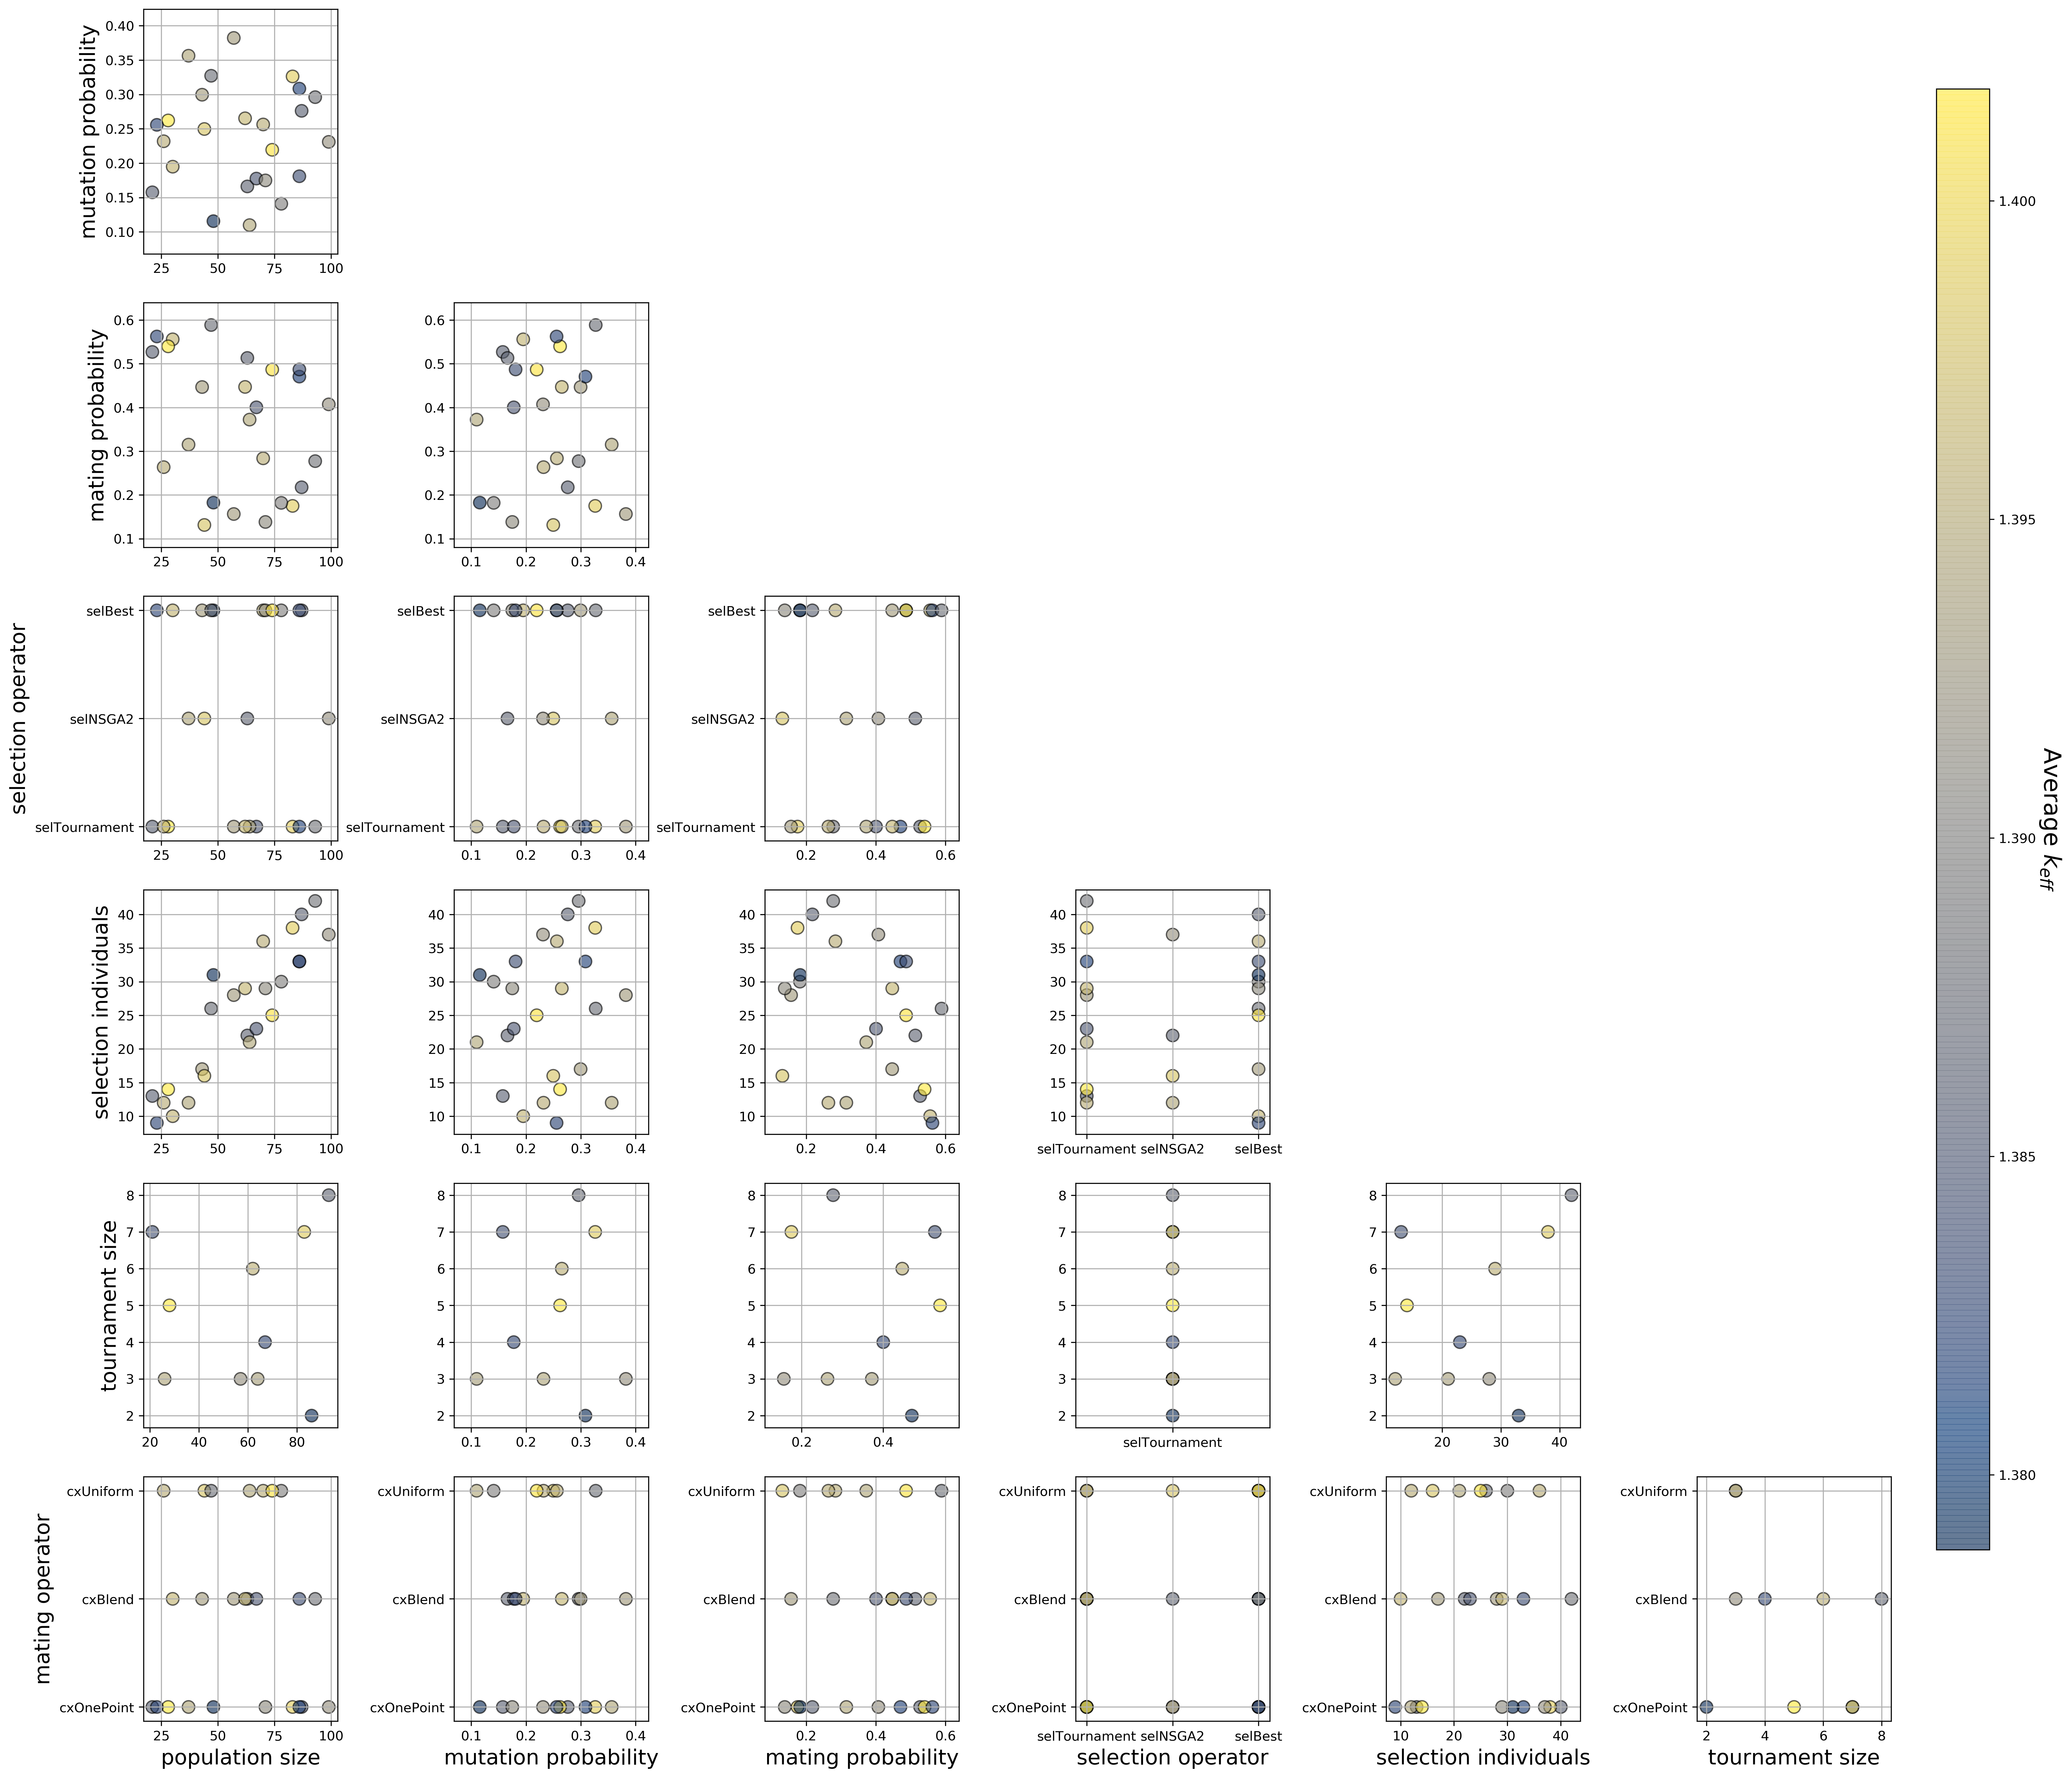
\includegraphics[width=1.3\linewidth]{hyperparameter_sens.png}} 
    \caption{Coarse hyperparameters search's results. Hyperparameter values are plotted 
    against each other with a third color dimension representing each experiment's 
    final population's $k_{eff ave}$.}
    \label{fig:hyperparameter_sens}
\end{figure}
I plotted the hyperparameters against each other to visualize the interdependence 
between hyperparameters. 
From the coarse hyperparameter search, I noticed the following trends: 
\begin{itemize}
    \item Mutation probability has a higher $k_{eff ave}$, between 0.2 and 0.4. 
    \item Mating probability has a higher $k_{eff ave}$, between 0.1 and 0.3. 
    \item Population size has a higher $k_{eff ave}$, between 20 and 60. 
\end{itemize}
There is also no interdependence between hyperparameters. 

Next, I proceeded to the fine searches. 
From Figure \ref{fig:hyperparameter_sens}, I narrowed down population size, 
mutation probability, and mating probability bounds, as shown in Table 
\ref{tab:hyperparameter_search}'s \textit{Fine Search 1 Bounds} column. 
I found no significant trends in the other hyperparameters, so I left them 
as is. 
I ran ten more experiments (25 to 34) sampling hyperparameters from 
the \textit{Fine Search 1 Bounds}. 
From these results, I conducted a second fine search with five experiments 
(35 to 39) with further tuned hyperparameter bounds, as shown in Table 
\ref{tab:hyperparameter_search}'s \textit{Fine Search 2 Bounds} column. 
I determined these new hyperparameter bounds based on these reasons: 
\begin{itemize}
    \item Mutation probability has a higher $k_{eff ave}$, between 0.2 and 0.3.
    \item I overlooked $k_{eff ave}$  peaking at mating probability between 
    0.45 and 0.6 in the previous \textit{Fine Search 1}, thus shifted the bounds. 
    \item The highest $k_{eff ave}$ occurred for \texttt{selTournament}. 
    \item I narrowed down mating operator options to \texttt{cxBlend} and 
    \texttt{cxOnePoint} since they had higher $k_{eff ave}$. 
    \item I selected arbitrary numbers for population size, 
    selection individuals, and tournament size since they did not 
    correlate with $k_{eff ave}$ values. 
\end{itemize}
Figure \ref{fig:input_hyperparameters_sens} shows the relationship between 
hyperparameter values and $a$, $b$, $c$ control parameters, final generation 
$k_{eff max}$, and final generation $k_{eff ave}$. 
The coarse experiments' scatter points are made $50\%$ transparent, while the fine 
experiments' scatter points are opaque. 
\begin{figure}[]
    \centering
    \makebox[\textwidth][c]{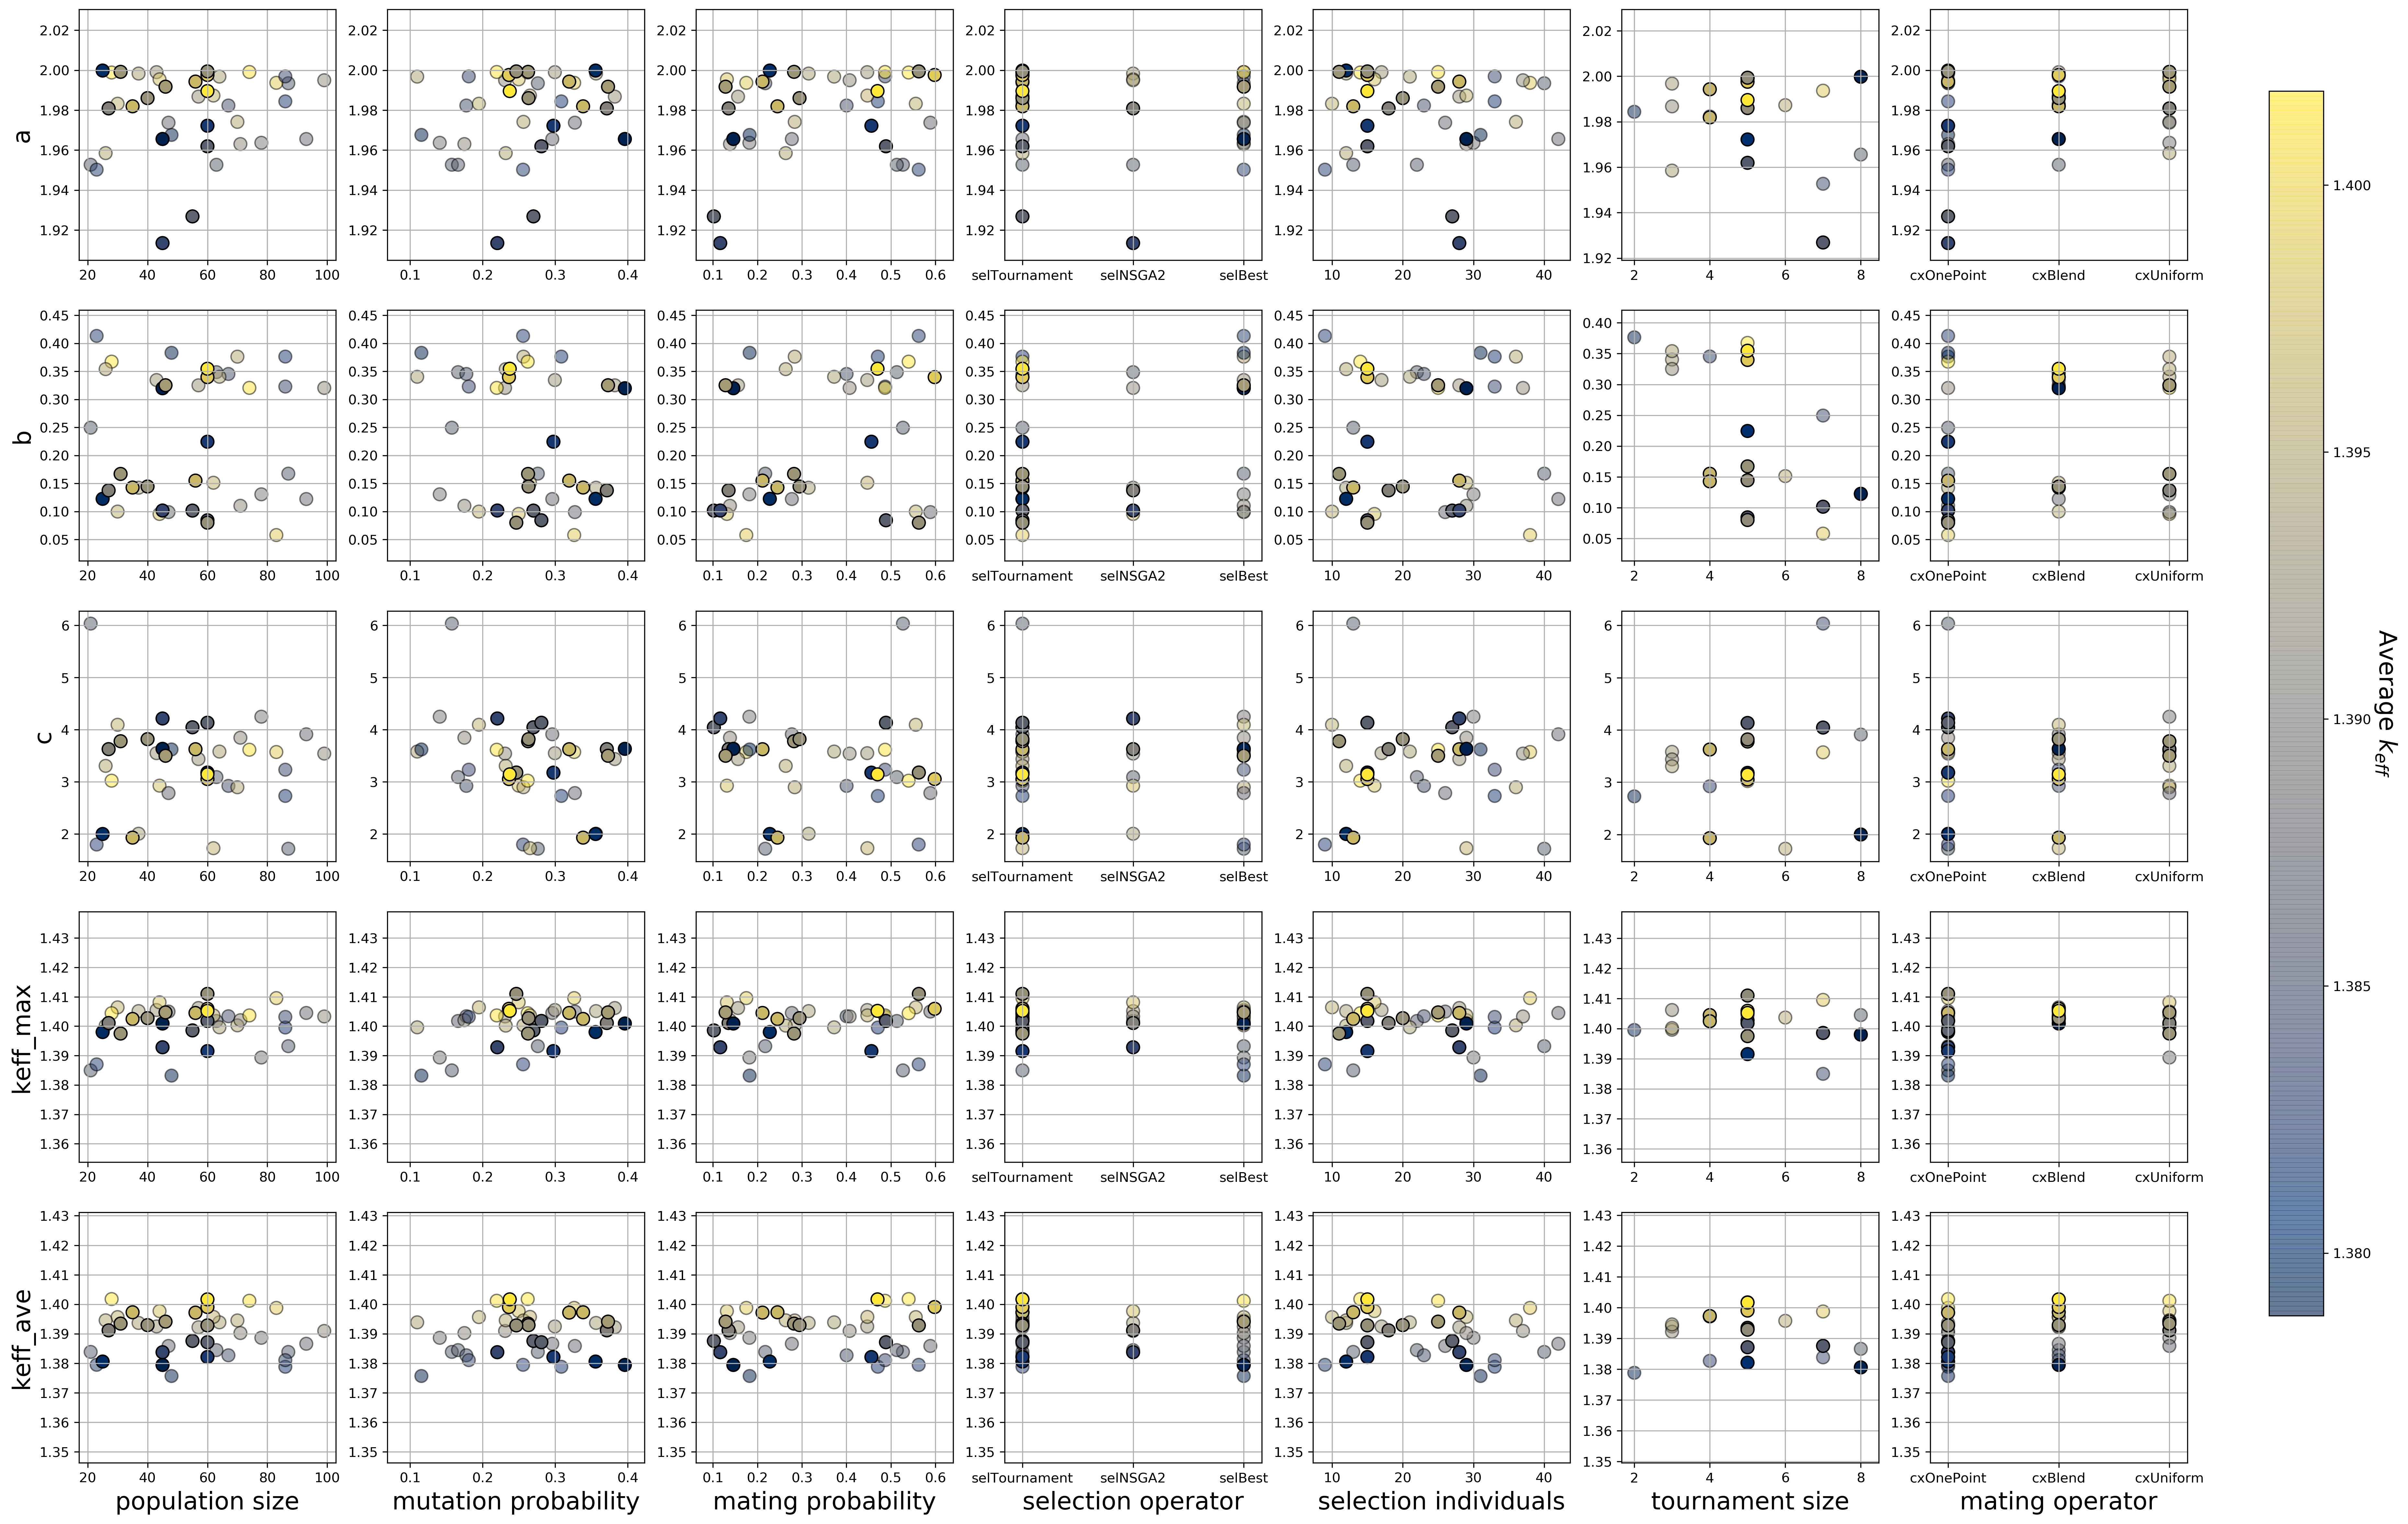
\includegraphics[width=1.3\linewidth]{input_hyperparameters_sens.png}} 
    \caption{Hyperparameters search's results for all 40 experiments (coarse 
    and fine). I plotted the hyperparameters against: a,b,c control parameters, 
    each experiment's final generation $k_{eff max}$, and final generation 
    $k_{eff ave}$ with a third dimension representing each experiment's final 
    population's $k_{eff ave}$. Coarse experiments' (0 to 24) scatter points 
    are $50\%$ transparent, while the fine experiments' (24 to 39) scatter points 
    are opaque. }
    \label{fig:input_hyperparameters_sens}
\end{figure}
In Figure \ref{fig:input_hyperparameters_sens}, on average, the fine experiments 
(opaque scatter points) have higher $k_{eff ave}$, which indicates that the
hyperparameter search process met its objective of finding hyperparameter 
bounds that enable quicker and more accurate optimization. 

Table \ref{tab:topfive} shows the hyperparameters for the five experiments 
with the highest final generation $k_{eff ave}$.
\begin{table}[]
    \centering
    \onehalfspacing
    \caption{Control Parameters, $k_{eff}$ results, and hyperparameter values for 
    the five hyperparameter search experiments with the highest final generation 
    $k_{eff ave}$.}
	\label{tab:topfive}
    \footnotesize
    \makebox[\textwidth][c]{\begin{tabular}{p{3cm}p{3cm}p{3cm}p{3cm}p{3cm}p{3cm}}
    \hline 
    \textbf{Control/Output Parameters}& \textbf{Experiment 6} & \textbf{Experiment 15} & \textbf{Experiment 24} & \textbf{Experiment 36} & \textbf{Experiment 39}\\
    \hline 
    $k_{eff ave}$ [-] & 1.39876 &1.40175&1.40118&1.39906&1.40165\\ 
    $k_{eff max}$ [-] & 1.40954 &1.40440&1.40365&1.40590&1.40519\\ 
    a [-] & 1.993&1.998&1.999&1.997&1.989\\
    b [$\frac{radians}{cm}$] & 0.057&0.367&0.320&0.339&0.354\\ 
    c [radians] & 3.571&3.022&3.615&3.053&3.143\\
    \hline
    \textbf{Hyperparameter}& &&&&\\
    Population size & 83 & 28&74&60&60\\ 
    Generations &8&22&9&10&10 \\
    Mutation probability & 0.32 &0.26&0.21&0.23&0.23\\
    Mating probability & 0.17 &0.53&0.48&0.59&0.46\\
    Selection operator & \texttt{selTournament} &\texttt{selTournament}&\texttt{selBest}&\texttt{selTournament}&\texttt{selTournament}\\
    Selection individuals & 38 &14&25&15&15\\
    Selection tournament size & 7 &5&-&5&5\\
    Mutation operator & \texttt{mutPolynomial} \texttt{Bounded}&\texttt{mutPolynomial} \texttt{Bounded}&\texttt{mutPolynomial} \texttt{Bounded}&\texttt{mutPolynomial} \texttt{Bounded}&\texttt{mutPolynomial} \texttt{Bounded}\\
    Mating operator & \texttt{cxOnePoint} &\texttt{cxOnePoint}&\texttt{cxUniform}&\texttt{cxBlend}&\texttt{cxBlend}\\ 
    \hline
    \end{tabular}}
\end{table}
Figure \ref{fig:topfiveplot} shows the packing fraction distributions that 
produced the $k_{eff max}$ from the top five experiments. 
\begin{figure}[]
    \centering
    \makebox[\textwidth][c]{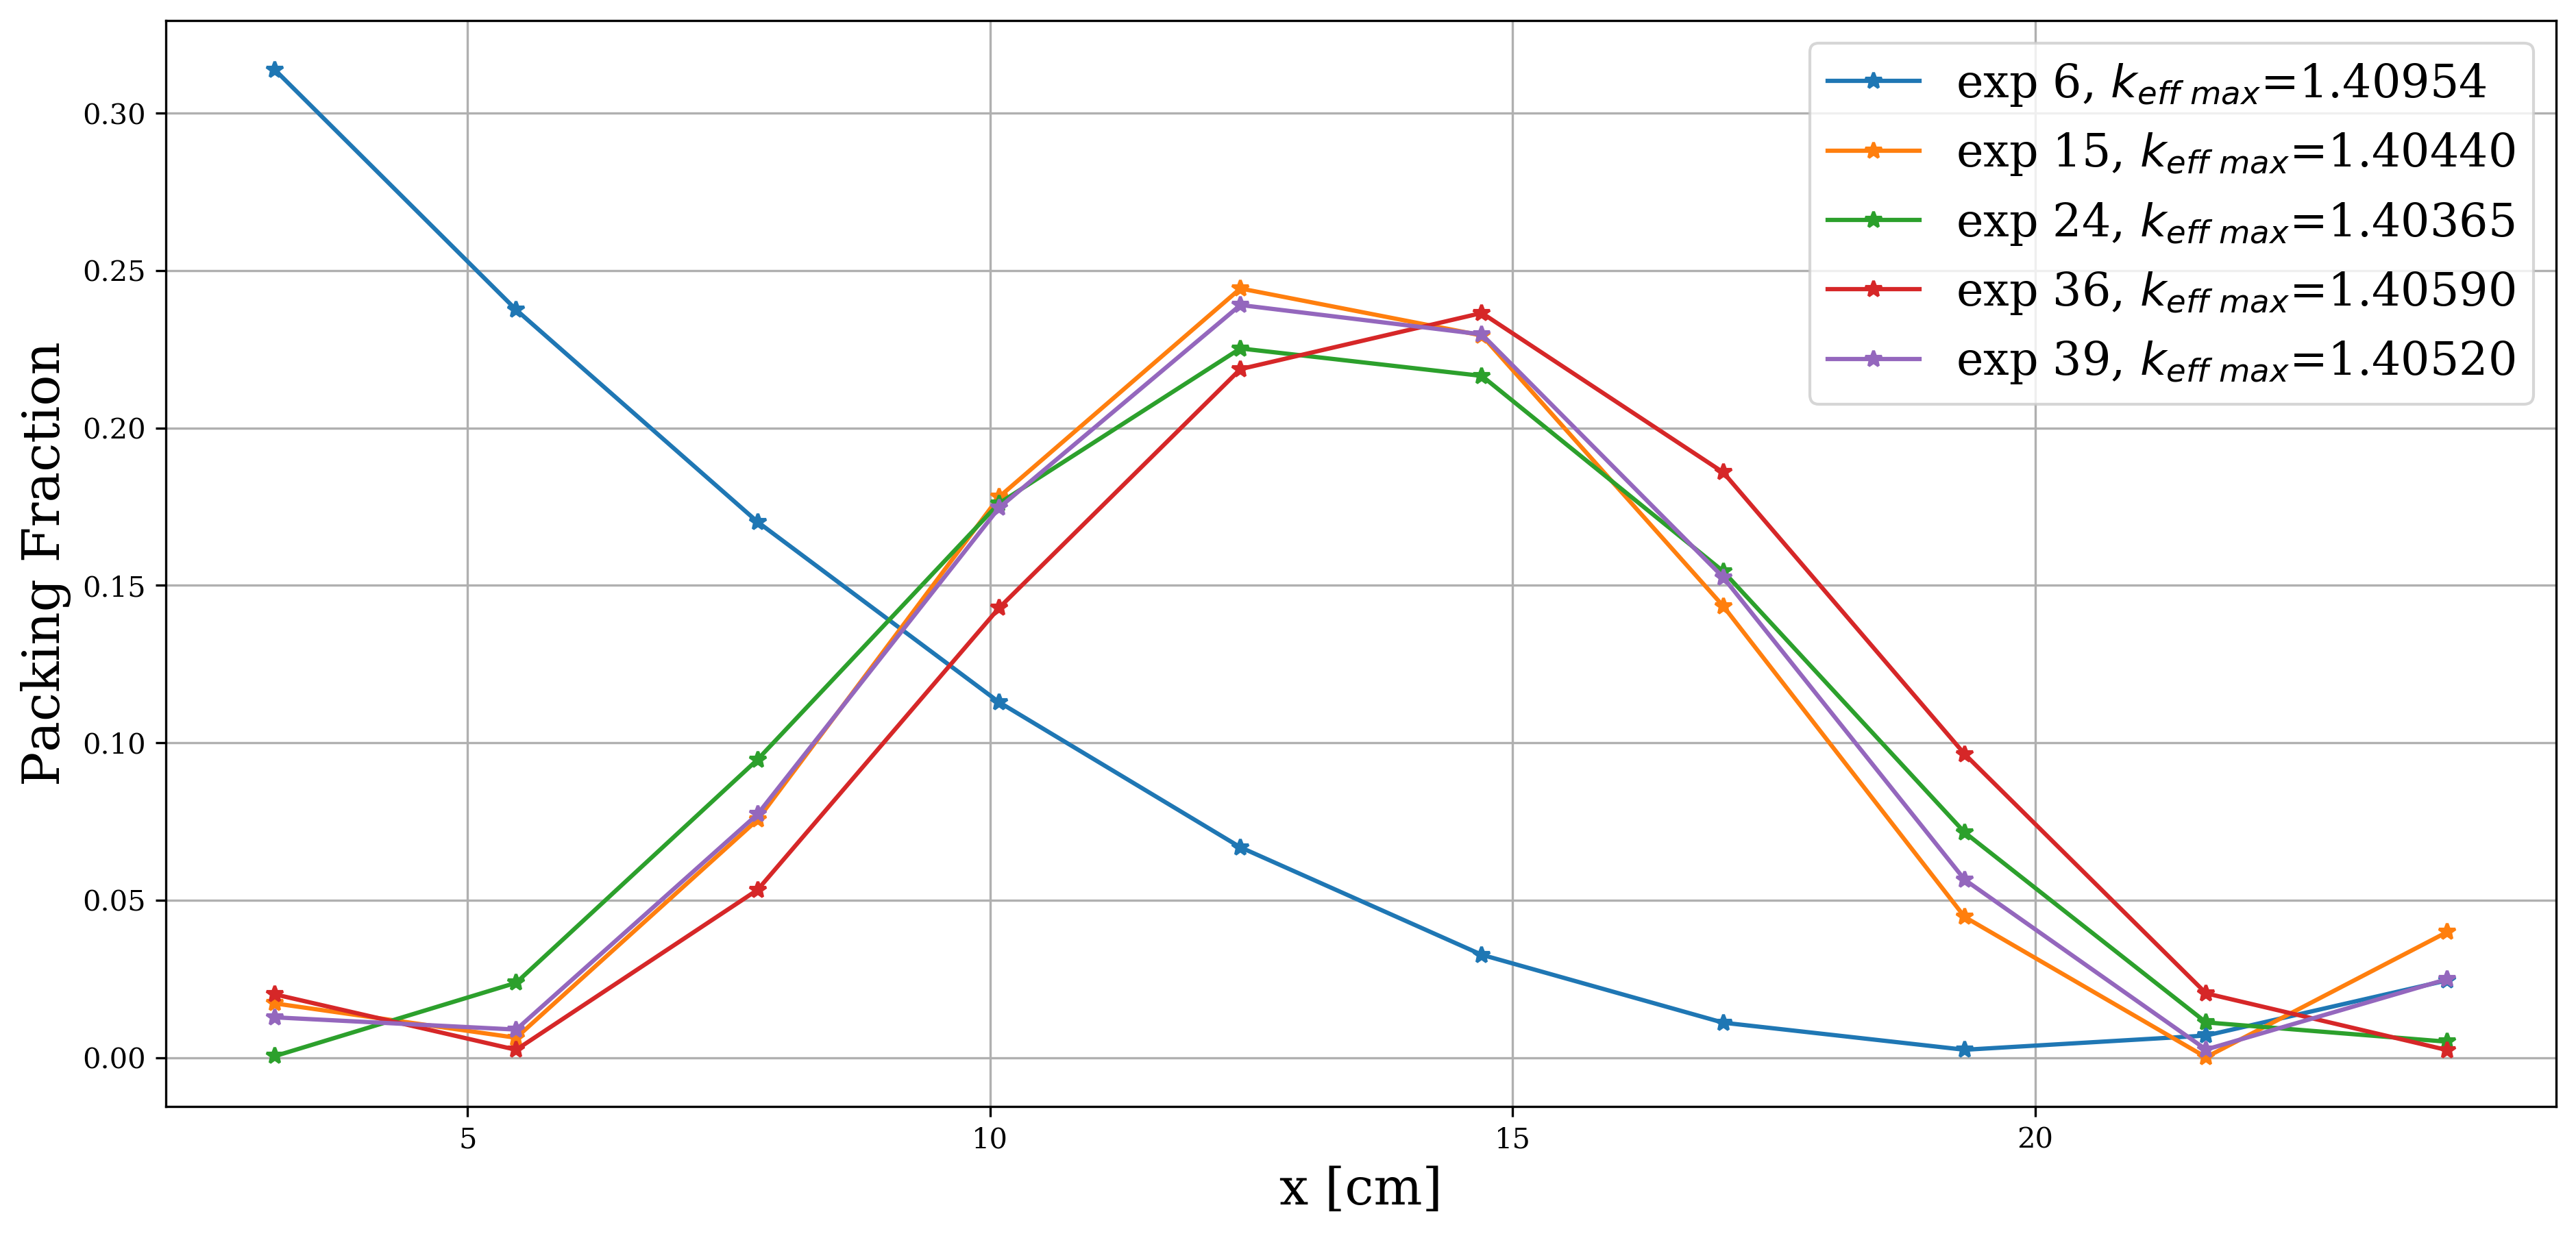
\includegraphics[width=1\linewidth]{topfive_plot.png}} 
    \caption{}
    \label{fig:topfiveplot}
\end{figure}
Four experiments had similar packing fraction distributions peaking at approximately 
0.23 in the slab's center, while one experiment had an exponential-like 
distribution with a peak packing fraction of 0.31 at the slab's side.
The similar final packing fraction distributions demonstrate genetic algorithms' 
robustness to find the optimal global solutions with different hyperparameters. 

I ran these simulations on the BlueWaters supercomputer \cite{ncsa_about_2017}. 
In each \gls{REALM} simulation, each generation runs a population size number 
of individual OpenMC simulations. 
Each OpenMC simulation takes approximately 13 minutes to run on a single BlueWaters 
XE node. 
With approximately 600 OpenMC evaluations per \gls{REALM} simulation, the total 
\gls{REALM} simulation takes about 130 BlueWaters node-hours. 
The hyperparameter search ran 40 \gls{REALM} simulations, thus using approximately
5200 node-hours.

\subsection{Results for Best Hyperparameter Set}
I define the best-performing hyperparameter set as the experiment that produces 
the highest $k_{eff ave}$ in its final generation. 
\textit{Fine Search 2}'s experiment 39 produces the best performing 
hyperparameter set, shown in Table \ref{tab:topfive}, with 
center-peaking packing fraction distribution with $k_{eff max} = 1.40519$. 
Experiment 39's $k_{eff max}$ exceeds the original straightened \gls{AHTR} 
configuration's $k_{eff}$ by $\sim2000$pcm. 
Figure \ref{fig:triso_distribution_sine_39} shows the packing fraction distribution 
that produced $k_{eff max} = 1.40519$. 
\begin{figure}[]
    \centering
    \makebox[\textwidth][c]{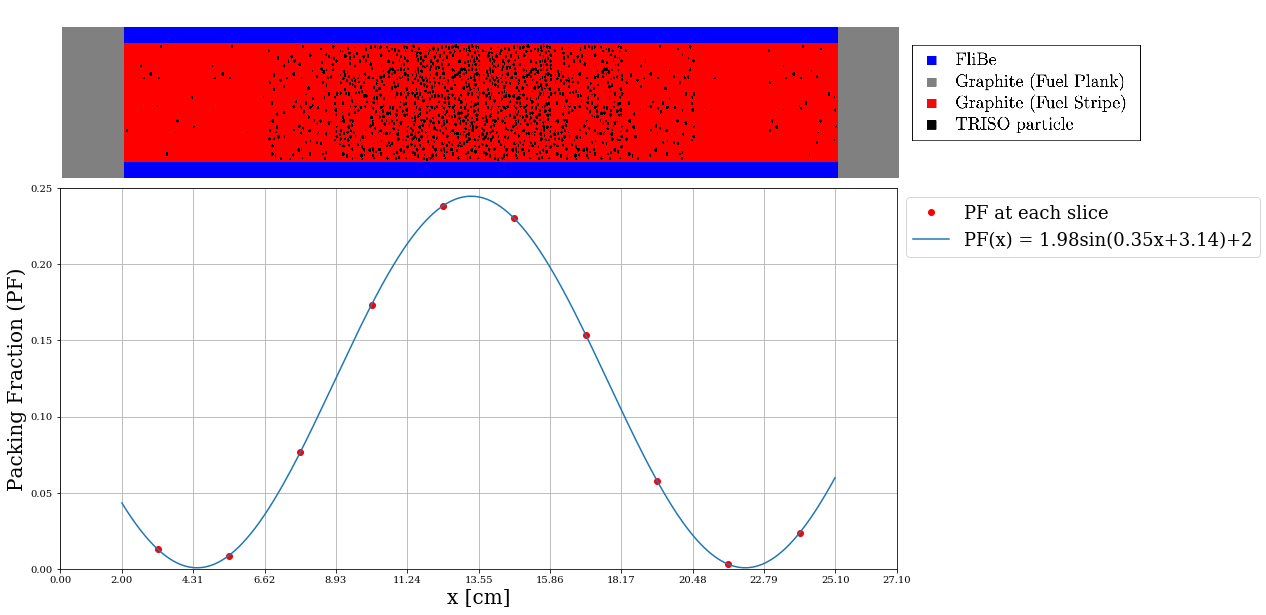
\includegraphics[width=1.1\linewidth]{triso_distribution_sine_39.png}} 
    \caption{Experiment 39 packing distribution that produced $k_{eff max} = 1.40519$. 
    Below: $PF(x) = (1.98\ sin(0.35x+3.14)+2)  \times NF$ sine distribution with 
    red points indicating the packing fraction at each slice. 
    Above: Straightened \acrfull{AHTR} fuel slab with varying \gls{TRISO} particle 
    distribution across ten slices based on the sine distribution. }
    \label{fig:triso_distribution_sine_39}
\end{figure}

Figures \ref{fig:keff_conv_39} and \ref{fig:pf_39} show the $k_{eff}$ evolution
and packing fraction distribution through the best performing 39$^{th}$ 
experiment's generations.
\begin{figure}[]
    \centering
    \begin{subfigure}{\textwidth}
    \makebox[\textwidth][c]{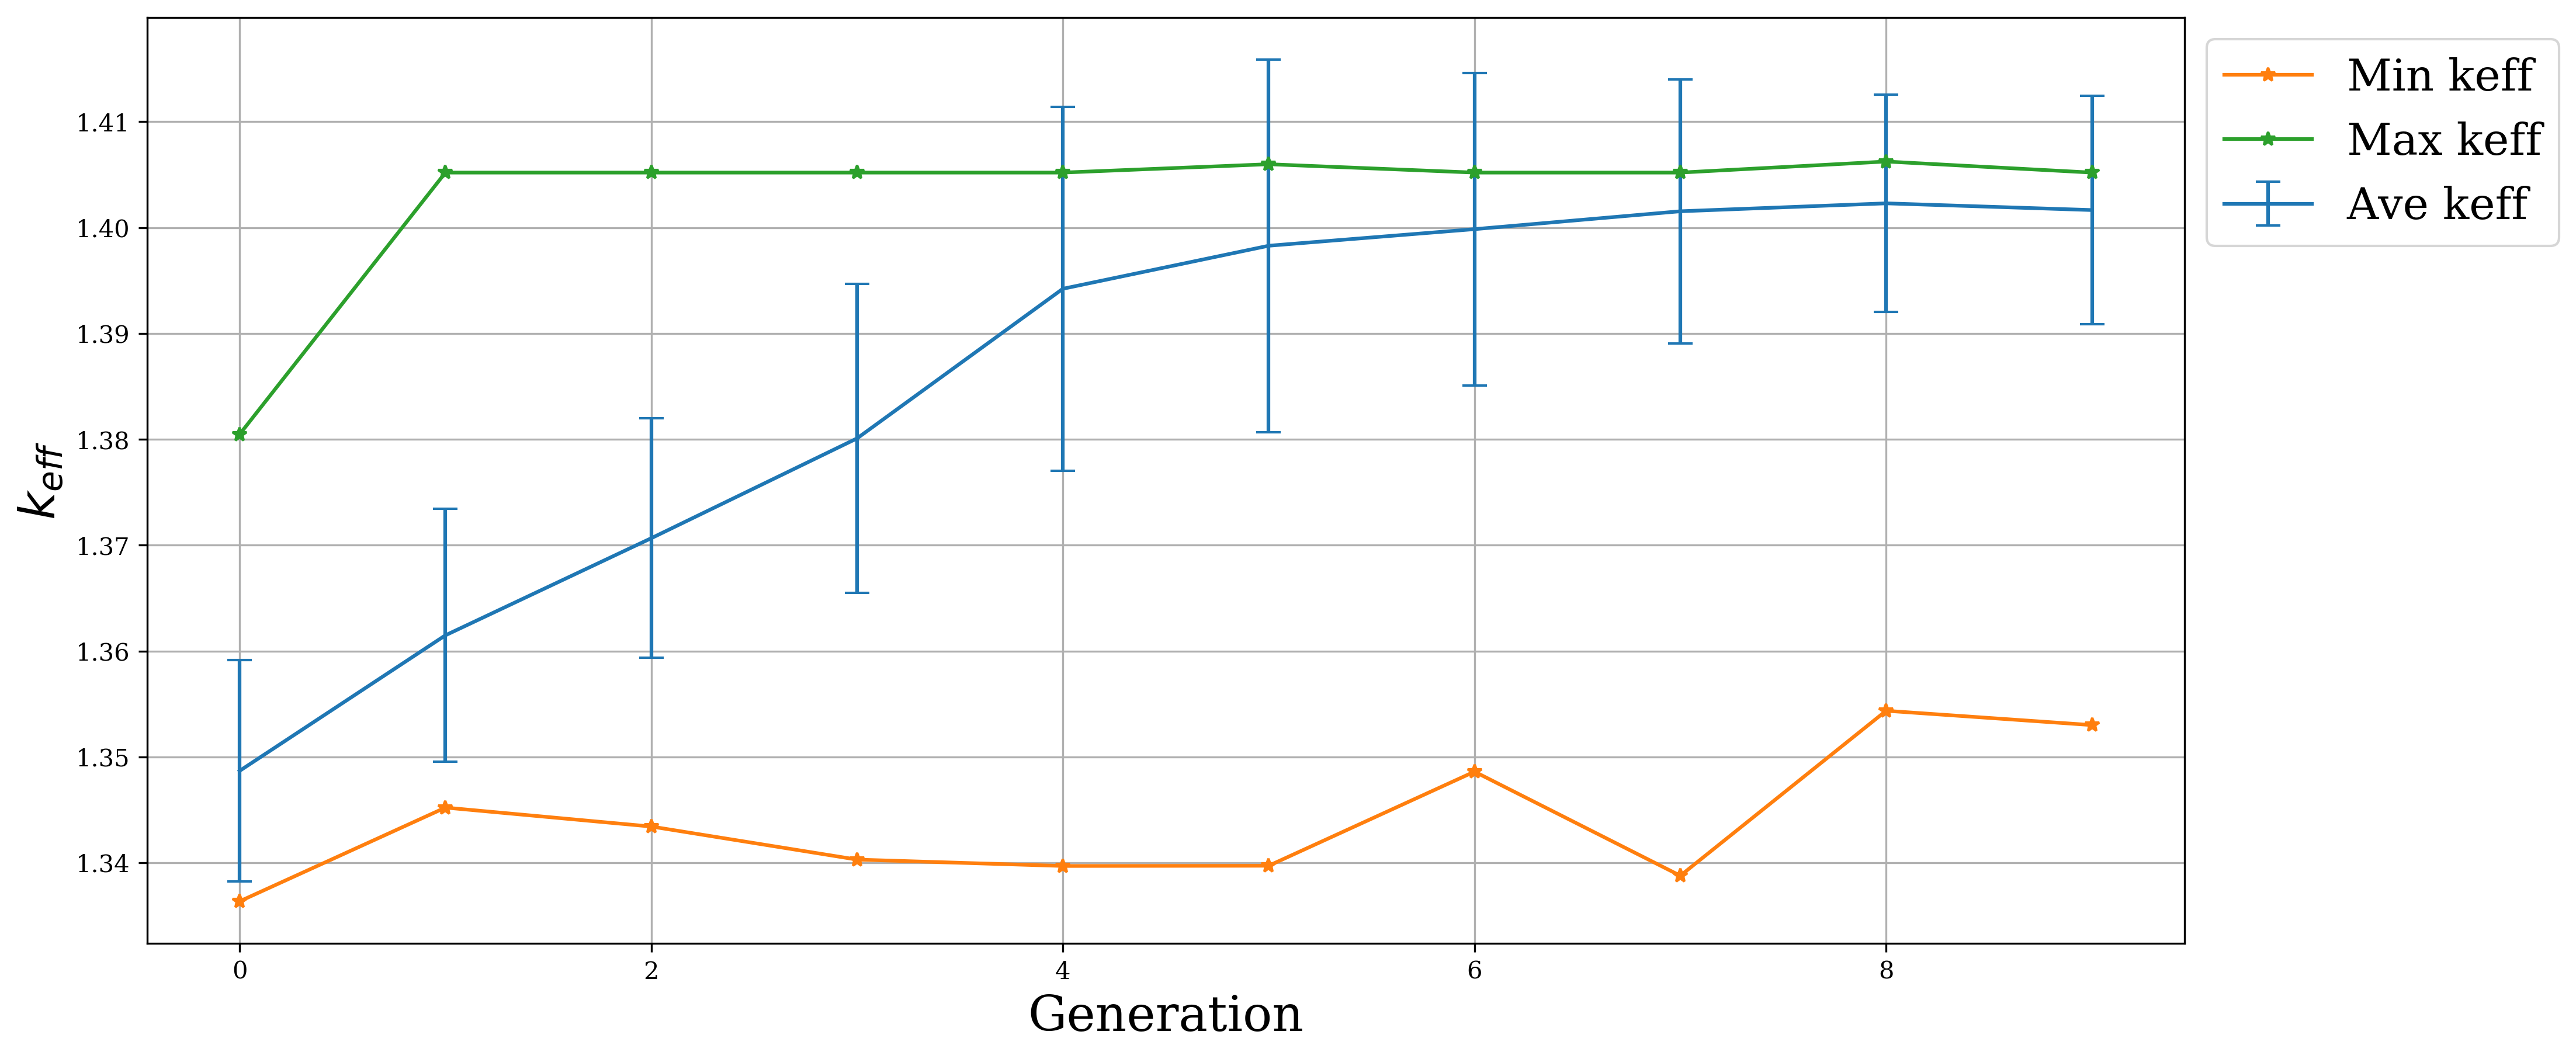
\includegraphics[width=1.1\linewidth]{keff_conv_39.png}} 
    \caption{Minimum, average, and maximum $k_{eff}$ values evolution.}
    \label{fig:keff_conv_39}
    \end{subfigure}
    \begin{subfigure}{\textwidth}
        \makebox[\textwidth][c]{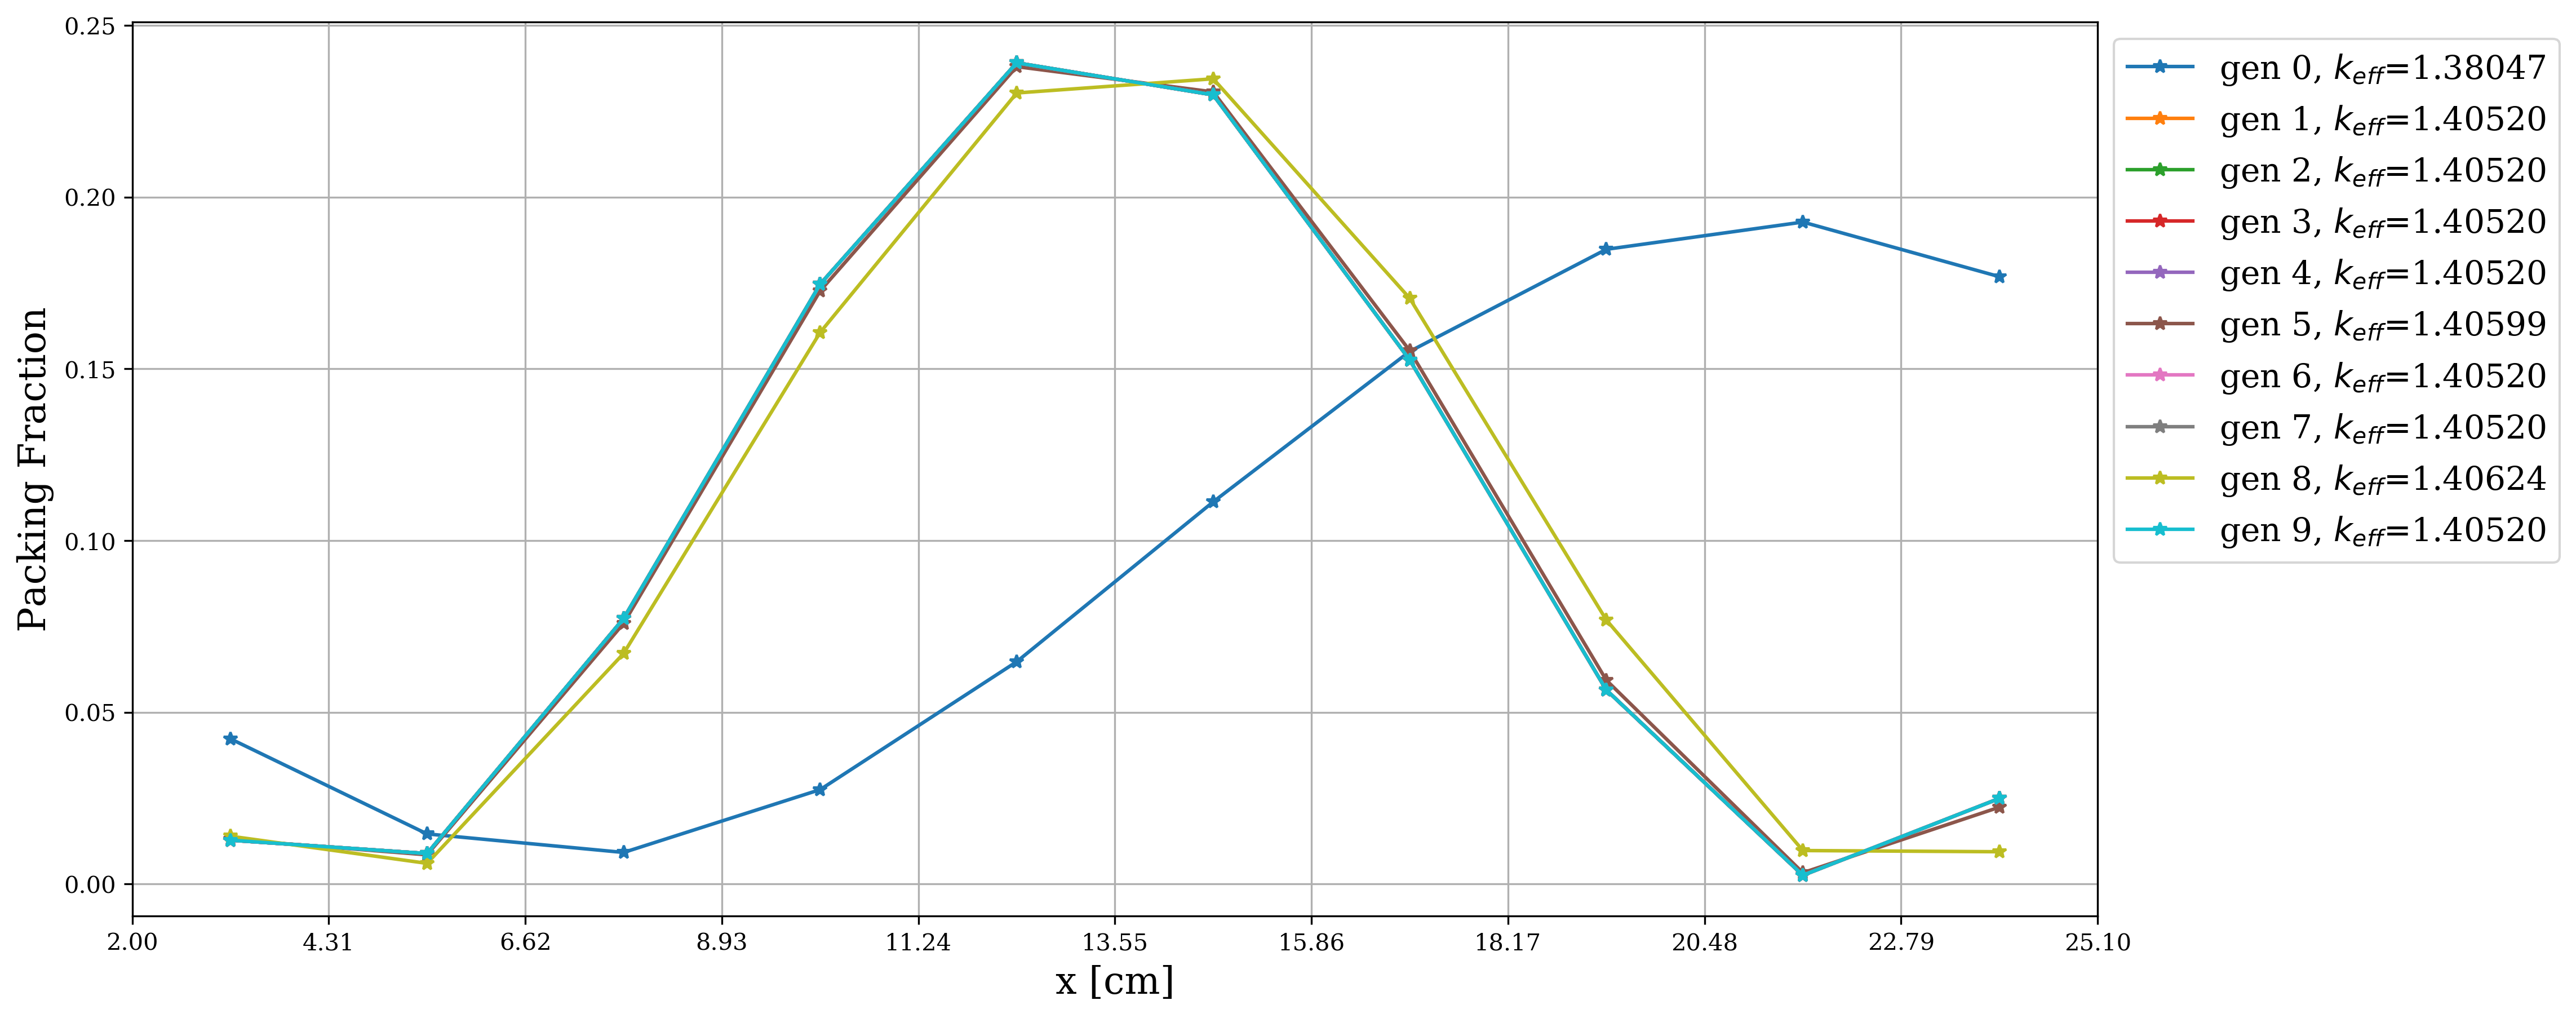
\includegraphics[width=1.1\linewidth]{pf_39.png}} 
        \caption{Maximum $k_{eff}$'s packing fraction distribution evolution.}
        \label{fig:pf_39}
    \end{subfigure}
    \caption{ Results for each generation for \gls{REALM}'s genetic algorithm optimization 
    of the Straightened \acrfull{AHTR} Fuel Slab. The \gls{REALM} simulation used 
    the 39$^{th}$ experiment's hyperparameter set.}
    \label{fig:39}
\end{figure}
The $k_{eff max}$ converged quickly by generation 1; however, this usually 
does not occur. 
The genetic algorithm optimizes stochastically, resulting in the possibility 
that the algorithm randomly samples a control parameter set that maximizes 
the objective function early in the optimization process. 
The $k_{eff ave}$ demonstrates how each generation's average $k_{eff}$
converges towards a higher value with each generation's improvements.
To demonstrate how the genetic algorithm optimization process usually goes, 
Figures \ref{fig:keff_conv_15} and \ref{fig:pf_15} show the $k_{eff}$ evolution 
and packing fraction distribution through the second-best performing 15$^{th}$ 
experiment's generations.  
Experiment 15 demonstrates how both maximum and average $k_{eff}$ converge
towards a higher $k_{eff}$ with improvements from each generation.
\begin{figure}[]
    \centering
    \begin{subfigure}{\textwidth}
    \makebox[\textwidth][c]{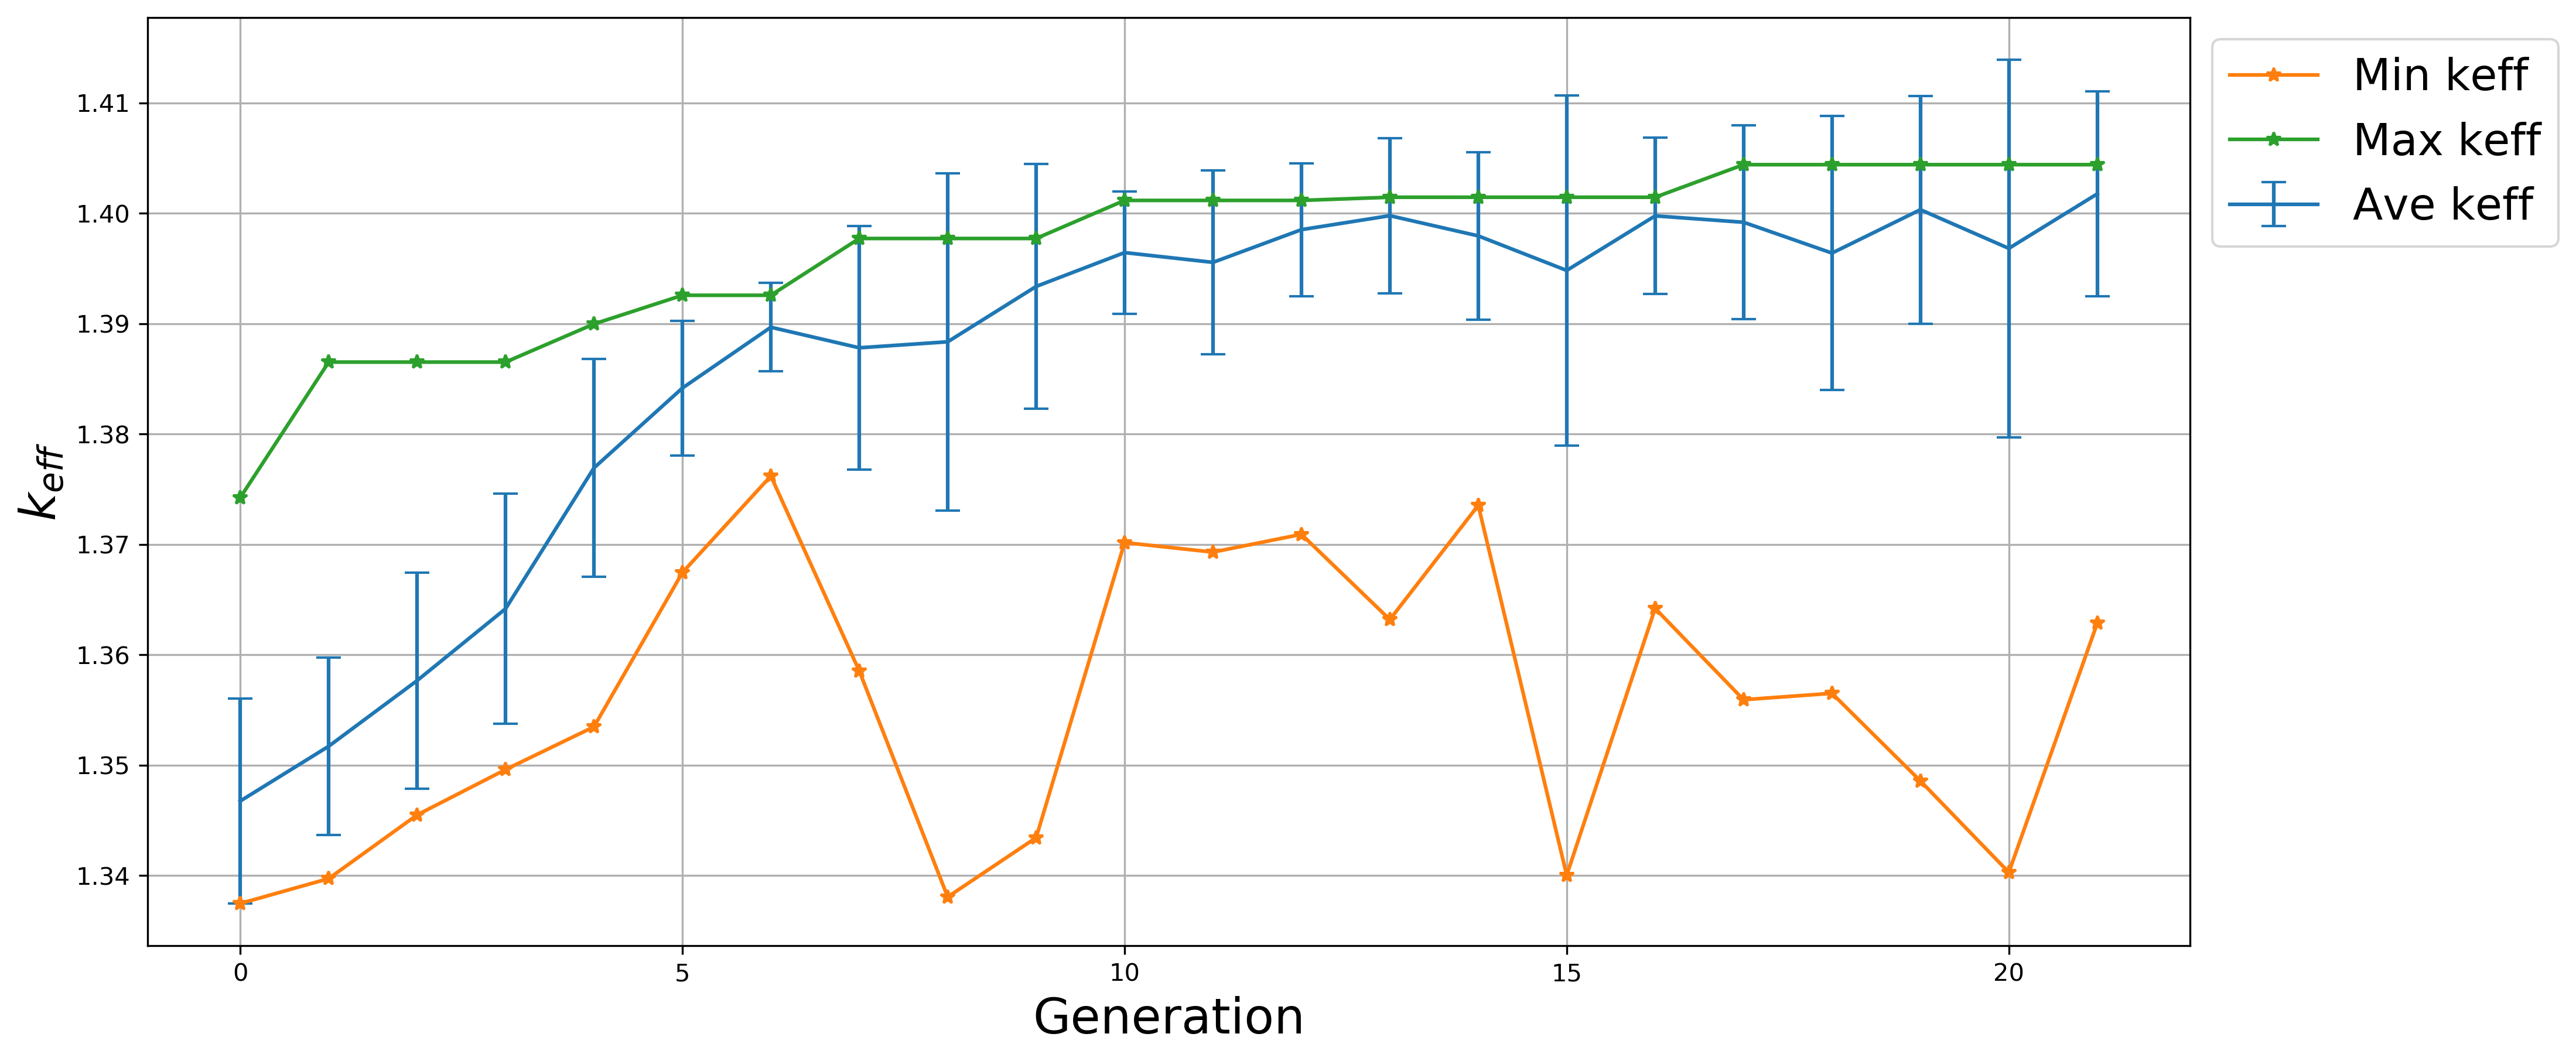
\includegraphics[width=1.1\linewidth]{keff_conv_15.png}} 
    \caption{Minimum, average, and maximum $k_{eff}$ values evolution.}
    \label{fig:keff_conv_15}
    \end{subfigure}
    \begin{subfigure}{\textwidth}
        \makebox[\textwidth][c]{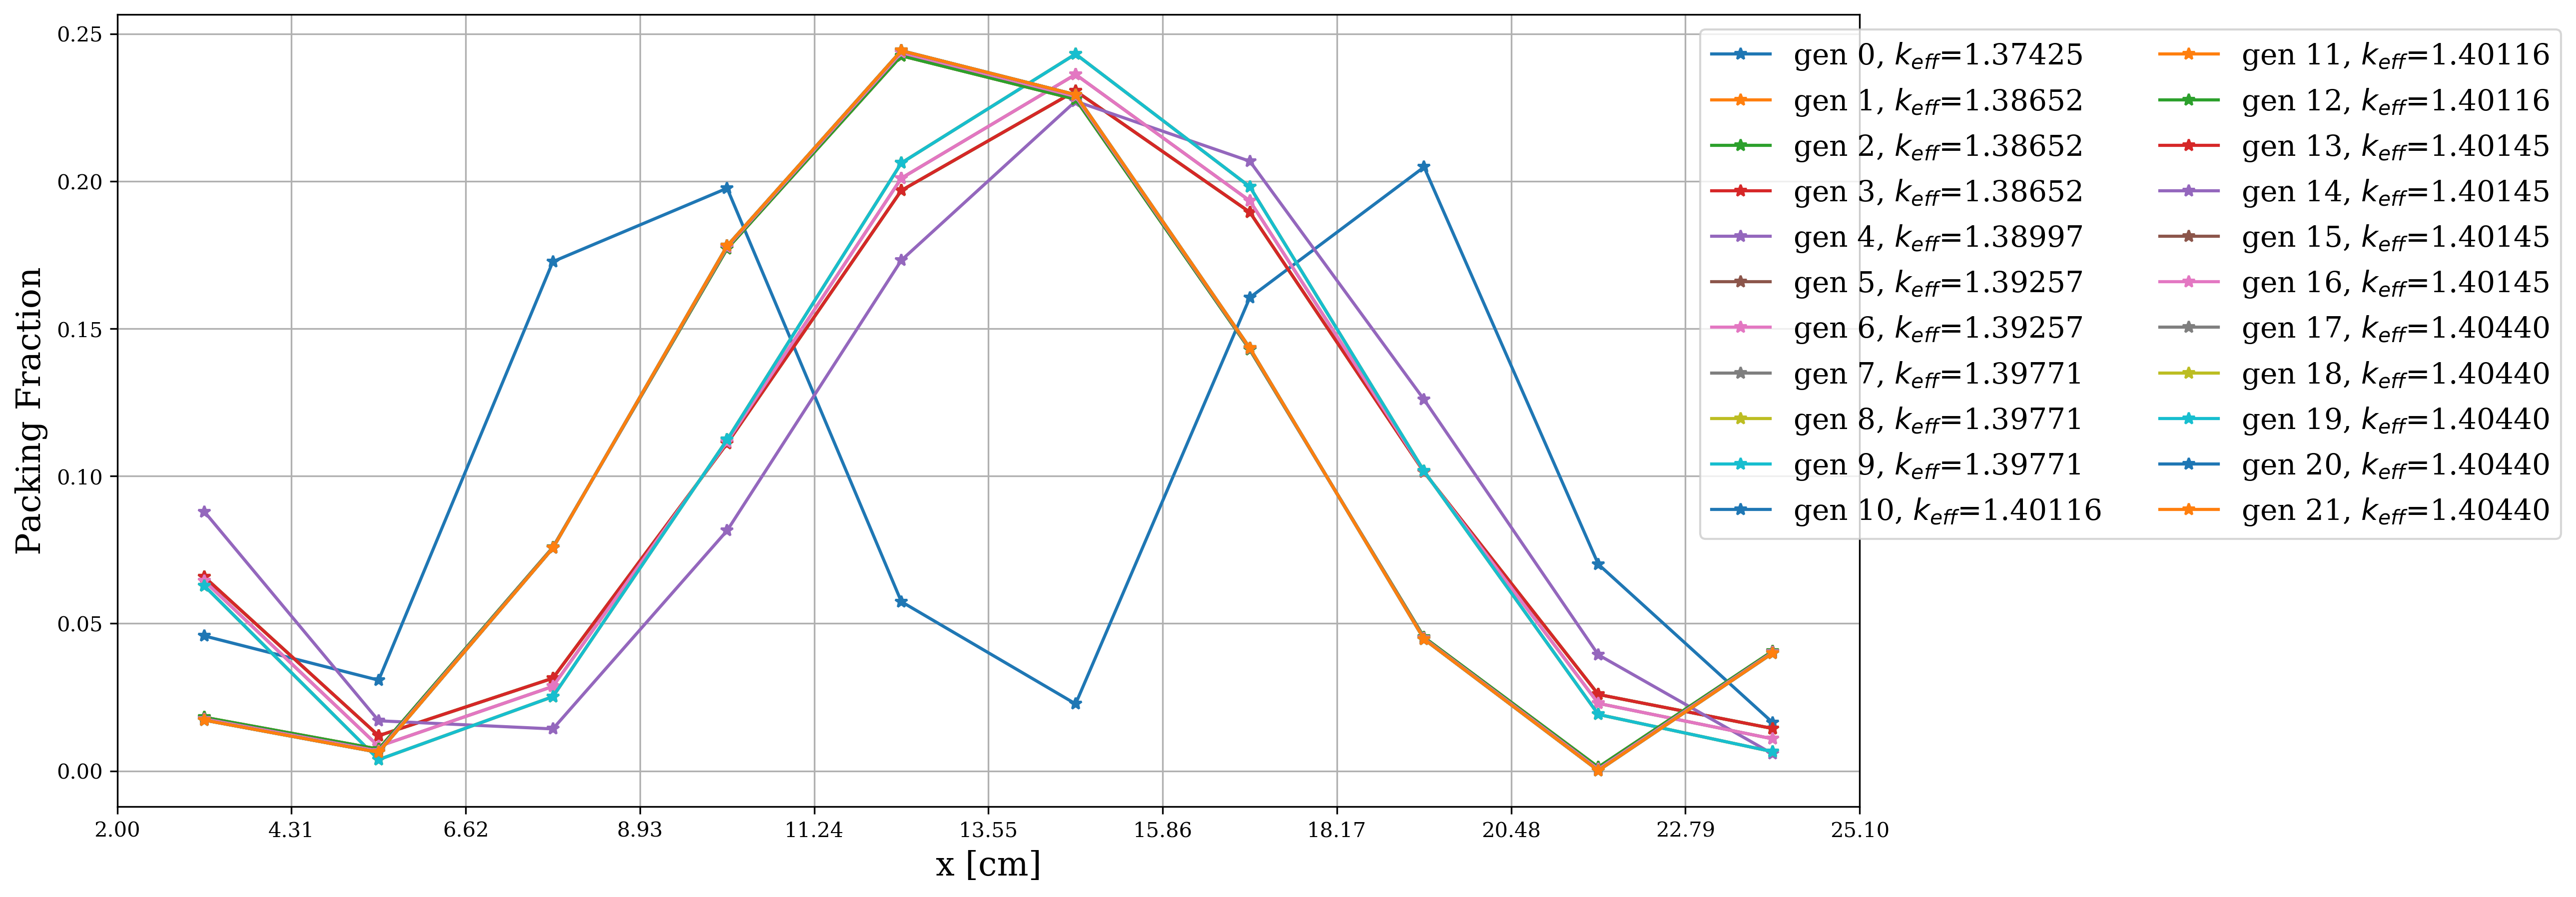
\includegraphics[width=1.1\linewidth]{pf_15.png}} 
        \caption{Maximum $k_{eff}$'s packing fraction distribution evolution.}
        \label{fig:pf_15}
    \end{subfigure}
    \caption{ Results for each generation for \gls{REALM}'s genetic algorithm optimization 
    of the Straightened \acrfull{AHTR} Fuel Slab. The \gls{REALM} simulation used 
    the 15$^{th}$ experiment's hyperparameter set.}
    \label{fig:15}
\end{figure}

Both Experiments 39 and 15 have packing fractions peaking at approximately 
0.23 in the slab's center and decreasing to zero at the slab's sides.  
The amplitude, $a$, for the packing fraction distribution that produced $k_{eff max}$ 
for Experiment 39 and the other top-five experiments (Table \ref{tab:topfive}) 
have settled at the upper bound of approximately 2. 
A higher amplitude, $a$, shows that a slab geometry with bigger packing fraction 
variations results in a higher $k_{eff}$. 
These observations about packing fraction distribution for $k_{eff max}$ are 
consistent with conclusions from the \gls{FHR} benchmark (Chapter 
\ref{chap:fhr-benchmark}): a high $k_{eff}$ occurs with a good balance between 
fuel loading and moderation space. 
Fission occurs at high \gls{TRISO} particle concentration areas at thermal flux;
however, the neutrons are born at fast-flux and require moderation to slow down 
to thermal ranges.
Therefore, larger moderation areas ensure higher resonance escape probability for 
the fast neutrons resulting in higher thermal flux, leading to more 
fission occurring and a higher $k_{eff}$. 

I also observed that \gls{TRISO} particle packing fraction peaks in the center 
of the slab, proving that if the optimization problem focuses purely on the slab's neutronics 
by maximizing $k_{eff}$, the fuel tends to culminate in the middle. 
This is nonideal for other important reactor core qualities, such as 
good heat transfer and ensuring flat power across the core. 
With these shortcomings in mind, I proceed to the future work chapter to discuss 
the proposed simulations that will optimize these other parameters. 

\section{AHTR Multiphysics Model Preliminary Work}
% compare TRISO particles 

\section{Summary}
This chapter demonstrated successfully applying \gls{REALM} to maximize $k_{eff}$ 
in a straightened \acrfull{AHTR} fuel slab by varying the \gls{TRISO} 
particle packing fraction distribution. 
I began by conducting a coarse-to-fine random sampling hyperparameter search to 
find the genetic algorithm hyperparameters that worked best for this optimization 
problem.
Experiment 39 performed the best with a hyperparameter set that produced the 
highest final generation $k_{eff ave}$ of 1.40165. 
The \gls{TRISO} particle packing fraction distribution that produced the final 
generation's maximum $k_{eff}$ of 1.40519 peaks at the slab's center with 
packing fraction distribution: $PF(x)=1.989\ sin(0.54x+3.143)$. 
This problem demonstrated the effectiveness and robustness of genetic algorithms 
at optimizing reactor parameters for an objective function. 
This demonstration problem had a single objective function, which was to maximize 
$k_{eff}$. 
However, many other objectives should be considered, such as maximizing heat 
transfer and minimizing power peaking in the core.
Thus, in the next chapter, I propose future simulations for optimizing
these objective functions simultaneously.
